\chapter{Metodolog\'ia y dise\~no de un experimento para inducir ansiedad en cuidadores de personas con demencia}\label{capit:cap3}
\vspace{-2.0325ex}%
\noindent
\rule{\textwidth}{0.5pt}
\vspace{-5.5ex}% 
\newcommand{\pushline}{\Indp}% Indent puede ir o no :p
\section{Introducci\'on}\label{secc:introduction}

Como vimos en el cap\'itulo 2, la mayor\'ia de los estudios logran inducir ansiedad o estr\'es por medio de situaciones controladas dentro del laboratorio exitosamente. Sin embargo, generar ansiedad en cuidadores informales es mucho mas dif\'icil: El escenario de un laboratorio no coincide con el entorno en el que una persona con demencia se desarrolla por lo que los comportamientos impredecibles no ser\'ian congruentes con el ambiente. Adem\'as, exponer a personas sin experiencia ante una persona con demencia que tiene necesidades reales resultar\'ia riesgoso para ambos individuos. Por otra parte, realizar una intervenci\'on totalmente natural a\~nade un grado de dificultad al estudio, resultando en ruido en los datos recolectados (p. ej. la se\~nal de ritmo card\'iaco podr\'ia ser alta no por una situaci\'on de ansiedad, sino por una actividad f\'isica, m\'ultiples distracciones o responsabilidades al mismo tiempo para el cuidador) haciendo d\'ificil de analizarlos para probar hip\'otesis.


[insertar imagen del triangulo de castro]
A continuaci\'on, se muestra un experimento que implementa la  t\'ecnica conocida como ``Naturalistic enactment (NE)'' \cite{Castro11}


\section{Un experimento para inducir ansiedad en cuidadores informales}
We designed an intervention to induce anxiety on informal
caregivers under controlled and naturalistic conditions.
To achieve this we applied a technique known as Naturalistic
Enactment (NE) \cite{Castro11}. NE was originally proposed
to evaluate pervasive healthcare technologies, where having
high ecological validity and direct user involvement is 
important, yet using actual patients can be risky. NE consists
of a naturalistic enactment of tasks (i.e. the exposure to 
situations and tasks in natural conditions) to simulate 
the experience of the user under normal conditions, and 
thus unearth issues and behaviors that would otherwise have
been difficult to capture. 

In order to ``expose'' our subjects to a realistic and
stressful caregiving situation under controlled conditions,
we conceived an exercise that consisted of a naturalistic
enactment of a therapy session with a person acting as being
a PwD. An elder of 75 years old acted as if she suffered
from mild dementia. She was trained with typical behaviours
such as: mumbling, screaming, wandering, repetitive questioning,
among others. She was already familiar with these behaviors
from acquaintances that suffer from dementia. The participants
were told that they would be working with a person who actually
suffers from dementia. Also, the real goal of the experiment
was not revealed. Instead, they were told that we were 
evaluating their performance as caregivers based on the 
initial training provided.

%Written consent was obtained from all participants
before the first session and a non disclosure agreement
was also signed to avoid the participants to talk to each
other about the experiment, the behaviors of the elder or
any techniques on how to handle the elder\textquotesingle s
behaviour, for as long as the experiment lasted.

\subsection{Subjects}
%The subjects were recruited by sending an email
to the University\textquotesingle s graduate students.
A compensation of two movie theater tickets was offered,
although many of them expressed interest in participating
despite of the prize. Participants were asked to participate
in 3 sessions (one per week), each one requiring approximately
90 minutes of their time. 

All the subjects participated in a training session, where we
explained the therapy activities they would have to perform
with the older adult.
Participants consisted of 10 graduate students (5 male,
5 female) with an average age of 24.7 (st dev. = 1.0593). 
Table 1 shows demographic data from the participants. 

\begin{table}[h]
\centering
\caption{Participants in the study.}
\label{Participants }
%\begin{tabular}{ |l>{\centering\arraybackslash}m{1in} |l>{\centering\arraybackslash}m{1in} |l>{\centering\arraybackslash}m{1in} |l>{\centering\arraybackslash}m{1in} l|}
\begin{tabular}{|c|c|c|c|c|}
\hline
 \textbf{Subject}&  \textbf{Gendre}&  \textbf{Age}&  \textbf{Caring Experince}  \\ \hline
 S1& Male & 24 & No   \\ \hline
 S2& Male &  25&  No  \\ \hline
 S3& Female & 24 & No   \\ \hline
 S4& Female & 26 & No  \\ \hline
 S5& Female & 24 & No   \\ \hline
 S6& Male & 26 &  No  \\ \hline
 S7& Male & 23 &  No \\ \hline
 S8& Male & 25 &  Yes  \\ \hline
 S9& Female & 26 & No   \\ \hline
 S10& Female & 24 & Yes  \\ \hline
\end{tabular}
\end{table}
\section{Procedure}
\subsection{Training}
All subjects participated in training session to familiarize 
them with the cognitive therapies they were going to be asked
to apply in the sessions with the older adult. The training
session lasted approximately 90 minutes, and all participants
practiced the therapies and had a chance to ask questions.
They were not given any strategies on how to cope with 
problematic behaviors from the older adult. Participants 
were told that the older adult had mild cognitive decline 
and could exhibit some behavioral problems such as forgetting 
recent instructions, apathy, unwillingness to complete the
task, etc. They were told that the tasks did not have to be 
completed if the older adult was not cooperating, but that they
should try to complete the therapy if possible. 
\subsection{Therapy tasks}
Before beginning the task, we equipped participants
with an electrical pulse reader (Zephyr Hxm) on the
chest to monitor heart rate, an Empatica E3 wristband 
to get Galvanic Skin Response and body temperature  
and a Muse band EEG monitor. All sessions were videotaped
for further analysis. 

For five minutes, and once instrumented, 
the subjects relaxed by concentrating on their
own breathing with eyes closed to obtain baseline
physiological data.	

Participants were asked to guide the older adult through
a therapy session which involved two of the 8 tasks that
were explained during the training session. Table 2
presents these tasks performed by each participant
in the three sessions of the study.

\begin{table}[h]
\centering
\caption{Therapies performed with the older adult by each
participant. }
\label{my-label}
\begin{tabular}{|c|c|c|c|c|}
\hline
 \textbf{Participant}&  \textbf{Therapy 1}& \textbf{Therapy 2}   & \textbf{Therapy 3}  \\ \hline
 S1&  Lace tying& Memory puzzle & Image classification   \\ \hline
 S2&  Image classification& Lace tying & Words puzzle   \\ \hline
 S3&  Words formation& Words puzzle & Memory puzzle    \\ \hline
 S4&  Lace tying& Image classification & Memory puzzle   \\ \hline
 S5&  Image classification&  Lace tying & Words puzzle   \\ \hline
 S6&  Objects separation& Memory puzzle & Lace tying   \\ \hline
 S7&  Objects separation & Lace tying & Words puzzle   \\ \hline
 S8&  Words puzzle& Lace tying & Image classification   \\ \hline
 S9&  Words formation& Image classificaton & Memory puzzle   \\ \hline
 S10&  Memory puzzle& Words formation & Lace tying   \\ \hline
\end{tabular}
\end{table}
%\begin{itemize}
%	\item Lace tying.
%%	\item Objects separation.
%	\item Memory puzzle.
%	\item Image classification.
%	\item Words formation with syllables.
%	\item Sentences with words.
%	\item Words formation.
%	\item Words puzzle.
%\end{itemize}

The whole intervention lasted 15 days, each participant
conducted a therapy with the older adult lasting approximately
30 minutes. Each day two participants assisted to the site. 

Each participant assisted to three sessions.
For each session, one or two tasks were made, with several
iterations in each task. None of the therapies were repeated
by participants. Also, none of the participants assisted with
the same partner more than once.

We divided the experiment in three weeks.
Each subject participated once every week.
We couched the older adult to enact different anxiety events.
First week, she acted levels from 0 to 2. In the second and 
third week, she acted levels from 0 to 3. In the last week,
we trained the participants to use coping strategies
(see Section 5).
\subsection{Setup}
We setted a room inside a real house to make it look as if
a person with dementia lived there. The customs included:
old furniture, low illumination, old pictures and paper 
hint tags over the hand washer. A wooden table was used 
to install the equipment: A Macbook, a Video Camera, and 
a smartphone to monitor the experiment. 

\begin{figure}[h]
        \centering
        \subfigure[]{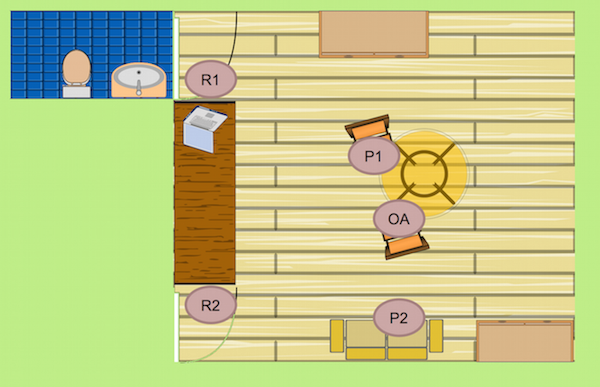
\includegraphics[width=160mm,height=80mm]{./Figures/img_exp_setup}}
        \caption{Experimental setup.
        The therapy activities were conducted
        on a table, with the PwD (OA) and the participant
        (P1) sitting facing each other. The second participant
        (P2) observed from the coah, while two researchers 
        (R1,R2) monitored the session from a nearby table.}
        \label{fig:img_exp_setup}
\end{figure}

Two researchers stood at the wooden table to
operate the equipment and take notes. We sat both
the participant and the elder face to face in a circular 
table. We asked the participants to use the bathroom to
wear the Zephyr band since it is worn under the clothes.
A second participant sat on a couch and we asked him to
observe the session. This participant was also being monitored
with a single empatica e3 wristband.

\subsection{Data gathering}
We developed two separate applications for the Empatica
E3 sensor and the Zephyr HxM band.
For the first device, we developed the 
``Care Me Too''  app for Android (see Figure 4) 
which connects to the E3 device via Bluetooth Low Energy,
displays the data in real time and saves it in .csv format. 
This aplication also can help to tag the events with user
input, making it useful for naturalistic studies.



\begin{figure}[h]
        \centering
        \subfigure[]{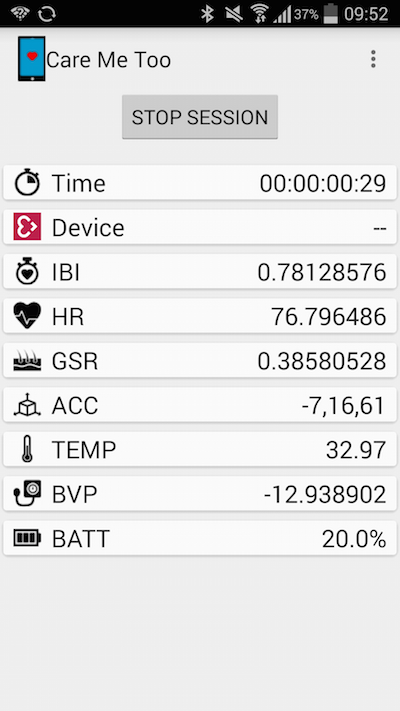
\includegraphics[width=160mm,height=80mm]{./Figures/img_caremetoo}}
        \caption{The Care Me Too App showing the physiological signals being recorded.}\label{fig:img_caremetoo}
\end{figure}

For the Zephyr HxM program, we used the anxiLogger
command line program (https://github.com/panzerfausten/anxiLogger) 
developed for an earlier study \cite{Miranda}.
The output .csv file was then appended to the Care Me Too
session data for timestamp synchronization
via a python library called ``maxiProcesser''.
(https://github.com/panzerfausten/maxiProcesser)
\\
For the Muse band we used the provided Muse lab
desktop application. The data was saved in a .muse
binary file and then exported to .csv plain text for
further analysis.
\\
We used a macbook laptop in site to connect the Zephyr
and muse devices, and a Samsung galaxy S4 for the E3
wristband to collect the data. Additional data of the
observer participant was also gathered. We did this by 
using a second Empatica E3 device in record mode wich
requires no additional bluetooth connection. 

\section{Data analysis and initial results}
All videos from the sessions were analyzed to segment
the events of interest, namely, when the older adult
enacted a behavior that could induce anxiety on the subject.
For instance, in one case the older adult, while engaged in
the therapy asks the subject: \textit{``Where is my mother?''}.
These segments where classified as one of three possible 
levels meeting our criteria (See table 3). Then, we took
a window of the corresponding GSR, HR,TEMP and EEG data 
and processed them individually.
\begin{table}[h]
  \caption{Event tagging criteria.}
    \begin{tabular}{|l|l|l|}
    \hline
    \textbf{Level} & \textbf{Criteria}                                                                                    & \textbf{Event Exmaple}                                                                      \\ \hline
    0     & \pbox{7cm}{PwD is passive,\\PwD is willing to participate,  \\Participant and PwD engaged with the task.} &                   \pbox{7cm}{The PwD performs the activity as \\requested}                       \\ \hline
    1     & \pbox{7cm}{Reluctant behaviours,\\Unwilling to participate,  \\Complaining about the task.}                & \pbox{7cm}{ ``I don t like this game'' \\ ``This is too hard'' \\``Do it your self'' }             \\ \hline
    2     & \pbox{5cm}{Mumbling,\\Talking nonsense,  \\Unpredictable behaviour.}                                      & \pbox{5cm}{``Where is my mother?''\\``Who are you?''}                                          \\ \hline
    3     & \pbox{5cm}{Shouting.\\Threatening the participant,\\Paranoia,  \\Urge to leave.}                          & \pbox{5cm}{``MOTHER, WHERE ARE YOU!!??''\\``I WANT TO LEAVE NOW!''  \\``WHO ARE YOU? LET ME GO!'' } \\ \hline
    \end{tabular}
\end{table}
\section{Configuraci\'on}

\subsection{GSR Pre-processing}
We developed a python library to process all the physiological
data, including export, feature extraction, timestamp 
synchronization, and plotting anxiety data from all the devices.


We started by downsampling the GSR data from 4.0 Hz to 1.0Hz
by calculating the average value of all the data falling 
into each 1 second window. This due we expected the anxiety
spans to last seconds. Then, we applied a gaussian filter to
smooth the signal and reduce noise. Finally, we used a python
scipy method to detect peaks and filtered all the peaks greater
to a threshold ( t >= 0.04 for not normalized data). 
We also calculated the ``Half Recovery Time'' of the signal.
That is, the point where the signals fall into the exact 
half of the peak value

This library also plots the data and can export the
GSR signal attributes (peaks, half recovery time, amplitude..)
into .csv and .json files which can be used for application
purposes.
	
\subsection{HR and IBI Pre-processing.}
Heart rate and InterBeat Interval (IBI) 
data was not necessary to down sample because
of the nature of the signal. The sensor only
reports data when the heart beat happens. However,
we did group it in windows of one seconds to compare
it with the rest of the signals. The data noise was
very low and it required no extra pre processing.
\subsection{Video processing.}
All the videos were transcripted with the f4 
transcription program for Mac Os X. Then, we generated 
video subtitles by taking the transcript timings and 
exporting them with a custom python script to a SubRip 
format (.srt) for ease of analysis.


\subsection{Data segmentation.}
In order to obtain ground truth, two researchers coded
the sessions live, by taking note of time, level of 
perceived anxiety, and a description of the event.

This description was noted by either what the participant 
and/or the elder said or did at the moment. Later,
we codified the videos by watching them and noting 
the timings and perceived anxiety level. This codification 
was made by two persons watching all the videos each.


The participants also had a paper form to indicate their
anxiety level after completing each iteration of the task,
they were also asked to report the time when an iteration
was initiated and completed. However, many of them found 
it difficult to report it, mainly because they were engaged 
with the activity. 
Once we tagged the segments with a perceived level of 
anxiety, we plotted the corresponding segment of all the
signals for visual interpretation and feature extraction.
\newpage
%%=====================================================

